%% -*- mode: latex; mode: auto-revert -*-
\maketitle

\begin{abstract}
  Basic document that demonstrates the {\LaTeX} build flow that I use as well as several quirks regarding specific packages.
\end{abstract}

\section{Example Section}
Claude Shannon wrote a good masters thesis while at \todo{Figure out where Shannon went to school...}some university~\cite{shannon1938}.
The thesis was really interesting\schuyler{What did he talk about?}.
Early work by George Boole laid the foundations of logic~\missingcitation.
Figure~\ref{fig-shannon} shows the realization of Boole's logical constructs in actual hardware.

\begin{figure}[h]
  \missingfigure{Add a figure that shows the mapping of logical constructs to circuit elements.
    Not sure how to do this, though.}
  \caption{hello.
    sukkit.}
  \label{fig-shannon}
\end{figure}

\section{Scripts}
I currently use one main script for keeping {\LaTeX} code in a \emph{nice} state for version control.
Specifically, I use a script, \texttt{fmtlatex}, to enforce a one-sentence-per-line rule on all files in the source directory that begin with \texttt{sec-}.
The included Makefile will, by default, run this on all source files that match this criteria.
I'm not dead-set that this is the right way to go about this, but it's how this is setup.
The Makefile can be modified, trivially, to use the \texttt{noformat-build} target instead of the \texttt{format-build} target which will not run \texttt{fmtlatex} on input source files.

\section{PGFPlots}
PGFPlots is an extremely versatile and useful, but has a ridiculously high learning curve.
It's highly advisable to use the \href{http://mirrors.ctan.org/graphics/pgf/contrib/pgfplots/doc/pgfplots.pdf}{PGFPlots manual} as a reference whenever designing these plots.
The colors that ship with PGFPlots are atrocious, however, and look terrible on a black and white printer.
I generally try to use a variety of colors, but to also use a variety of lightnesses to preserver some semblance of the original plots when printed on a terrible black and white printer.
\href{http://colorbrewer2.org/}{Colorbrewer} provides a good jumping off point for this for single hue colors.
In this directory, I include a forked submodule, \texttt{palette-art}, which generates a {\TeX} input file that defines all the colorbrewer colors.

\begin{figure}[h]
  \centering %% Example plot use tikz/pgfplots taken from the pgfplots manual

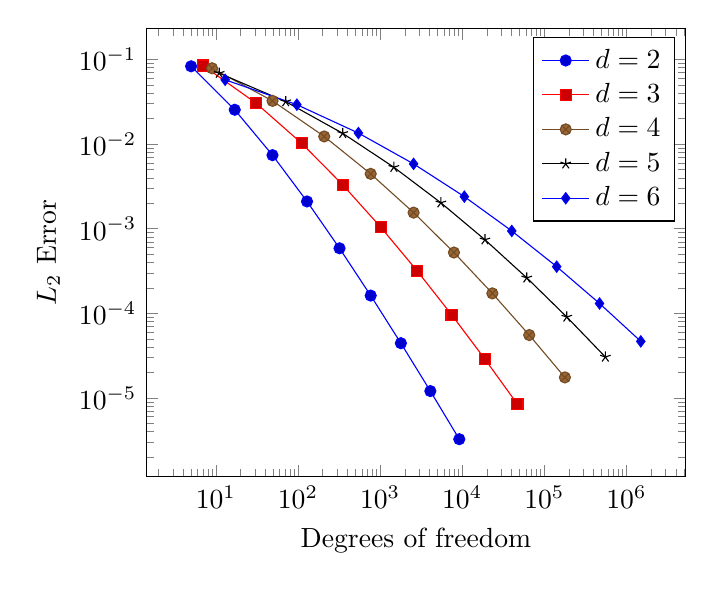
\begin{tikzpicture}
  \begin{loglogaxis}[
      xlabel={Degrees of freedom},
      ylabel={$L_2$ Error}
    ]
    \addplot coordinates {
      (5,8.312e-02)
      (17,2.547e-02)
      (49,7.407e-03)
      (129,2.102e-03)
      (321,5.874e-04)
      (769,1.623e-04)
      (1793,4.442e-05)
      (4097,1.207e-05)
      (9217,3.261e-06)
    };
    \addplot coordinates{
      (7,8.472e-02)
      (31,3.044e-02)
      (111,1.022e-02)
      (351,3.303e-03)
      (1023,1.039e-03)
      (2815,3.196e-04)
      (7423,9.658e-05)
      (18943,2.873e-05)
      (47103,8.437e-06)
    };
    \addplot coordinates{
      (9,7.881e-02)
      (49,3.243e-02)
      (209,1.232e-02)
      (769,4.454e-03)
      (2561,1.551e-03)
      (7937,5.236e-04)
      (23297,1.723e-04)
      (65537,5.545e-05)
      (178177,1.751e-05)
    };
    \addplot coordinates{
      (11,6.887e-02)
      (71,3.177e-02)
      (351,1.341e-02)
      (1471,5.334e-03)
      (5503,2.027e-03)
      (18943,7.415e-04)
      (61183,2.628e-04)
      (187903,9.063e-05)
      (553983,3.053e-05)
    };
    \addplot coordinates{
      (13,5.755e-02)
      (97,2.925e-02)
      (545,1.351e-02)
      (2561,5.842e-03)
      (10625,2.397e-03)
      (40193,9.414e-04)
      (141569,3.564e-04)
      (471041,1.308e-04)
      (1496065,4.670e-05)
    };
    \legend{$d=2$,$d=3$,$d=4$,$d=5$,$d=6$}
  \end{loglogaxis}
\end{tikzpicture}

  \caption{Example PGFPlots figure}
\end{figure}

\begin{table}
  \begin{tabular}{ll}
    \toprule
    foo & bar \\
    \midrule
    foo & bar \\
    \bottomrule
  \end{tabular}
  \caption[A ``good'' table]{Example of a ``good'' table that uses toprule, midrule, and bottomrule.}
\end{table}
